%%%%%%%%%%%%%FIX EQUATION NUMBERING !!!


\chapter[Accelerating structures]{Accelerating structures}

The accelerating structures are one of the key part of a particle accelerator. Even though in the first accelerators the particle acceleration was achieved simply with fixed fields, this technique showed its limitations quite soon due to the impossibility to create arbitrary high DC voltages without incur in electrostatic discharges. The present conventional technology for particle acceleration is based on the RF cavities, so it is natural try to push the state-of-the-art technology the further possible in order to reach the highest acceleration possible in the shortest length. In the case of the CLIC project a key issue is to be able to produce cavities with an accelerating field of 100 MV/m, which is the cutting-edge value at the moment when keeping the breakdown rate limited.

In this chapter some topics about the theory of accelerating cavities will be presented, the aim is to give to the reader a theoretical introduction to be able to understand the description of the cavity under test at the end of the chapter.

\section[Travelling wave accelerating structures]{Travelling wave accelerating structures}

In this section some useful concepts and result of the electromagnetic theory will be recalled. Because of conciseness, the examples and the geometries presented will refer to the travelling wave accelerating structures, since is the only type of structure relevant for the successive development of this work. The curious reader can find details on the untreated topics in \cite{Weiss:261732,Wangler:RF_LINAC,Humphries:107756} and in plenty of specialised books.

\subsection[Synchronous particle acceleration]{Synchronous particle acceleration}

A particle injected in an electromagnetic field in some conditions can gain energy at expenses of the field, getting accelerated. This is possible if the particle is injected at the right moment and the field and the particle have the same speed. In this manner the particle can travel with the field with an energy gain given by
\begin{equation}
\Delta W = q V_o cos \phi
\end{equation}
where $q$ is the charge of the particle, $V_0$ is the accelerating field and $\phi$ is the relative phase between particle and RF field.

In order to deliver a  constant energy gain to a charged particle it is necessary to shape the EM field matching  two fundamental conditions:

\begin{enumerate}
\item The electromagnetic wave has to have a non-zero component in the direction of the motion of the particle
\item The phase velocity of a wave has to be the same of the particle velocity, in order to keep the relative phase constant, and so the acceleration
\end{enumerate}
using some results of the theory of EM waves it is possible to show that the two condition cannot be met in the free space, but is necessary to build up some particular structures in order to coerce the electromagnetic field to propagate in the desired form. This is realised building particular structures that are similar to traditional waveguides, but presenting a lower phase velocity in order to make the synchronous acceleration possible.


\subsection[Reminder of Electromagnetism]{Reminder of Electromagnetism}

\subsubsection{Maxwell's equations}

It's well known since the basic courses of physics that the propagation of the electromagnetic fields follow the Maxwell's equations, that in a medium are

\begin{equation}
\begin{aligned}
\nabla . \vec{D} = \rho_{free}\\
\nabla . \vec{B} = 0\\
\nabla \times \vec{E} = - \frac{\partial \vec{B}}{\partial t}\\
\nabla \times \vec{H} = \vec{J}_{cond} + \frac{\partial \vec{D}}{\partial t}
\end{aligned}
\end{equation}
%%%%%%%%%%%%%%%STILL TO FIND A WAY TO ALIGN IT TO THE RIGHT
where $\vec{E}$ and $\vec{B}$ are the electric and magnetic field in the vacuum, $\vec{D} = \epsilon \vec{E}$, $\vec{B} = \mu \vec{H}$ and $\vec{E} = \sigma \vec{J}$. The propagation in vacuum is described by the same equations and can be easily derived with an appropriate choice of the constants.

\subsubsection[Waveguides and resonant cavities]{Waveguides and resonant cavities}

In some particular cases the confined propagation of electromagnetic waves is possible, and is commonly realised using a metal waveguide to direct all the energy in a single direction. In this section some useful results on the propagation in a waveguide will be stressed, the full derivation can be found in literature \cite{Botta:EM, Jackson:ClassEM,Weiss:261732}. 

The request of propagation in the direction of the axis of the waveguide can be traduced to the condition $\vec{E} \times \vec{n} = 0$, that means asking that no power is dissipated in the walls of the cavity by Joule effect since the electric field is normal to the surface anywhere and anytime.

Many solutions can be found to the problem, integrating the Maxwell's equations with the given boundary condition, but without entering in the calculations, the interesting solutions belong to two classes:
\begin{itemize}
\item \textbf{TM modes:} Transverse Magnetic modes, where the axial component of the magnetic field is null
\item \textbf{TE modes:} Transverse Electric modes, where the axial component of the electric field is null
\end{itemize}
where every mode has a particular cutoff frequency, and will propagate a wave only in case that the condition $\omega > \omega_c$ is met (where $\omega_c = 2\pi f_c$ and $f_c$ is the cutoff frequency of the mode). The cutoff frequency of each mode depends mainly by the geometry of the guide utilised, and waves with a frequency lower than the cutoff frequency will be exponentially damped.

For particle acceleration purposes, the fundamental feature of a waveguide is that the \textit{phase velocity} is $v_p = \frac{\omega}{k} > c$, so it's not suitable for particle synchronous acceleration. That's not surprising and can be understood with simple geometrical considerations\cite{Weiss:261732}, furthermore in principle there is no reason to put an upper limit to the phase velocity, since the phase is a geometrical physical quantity. The dispersion relation for a uniform waveguide can be expressed as 
\begin{equation}
\omega^2 = \omega^2_c + (k_0 \, c)^2
\end{equation}
where $\omega_c = K \, c$ and $K$ is the cutoff wavenumber.

The \textit{group velocity} instead is $v_g = \frac{\partial w}{\partial k} < c$ as expected for the physical quantity representing the speed of propagation of the EM wave according to Relativity. 
In any case, waveguides are a key building block of particle accelerators to deliver the RF power form the production equipment to the accelerating cavities.

A particular case is represented by the \textit{Resonant Cavities}, which are closed waveguides at the terminations (e.g. a cylindrical cavity, or \textit{pillbox cavity}, is composed of a circular waveguide closed by two planes at the extremities). In the resonant cavities the EM field can resonate according to the peculiar eigenfrequencies of the system, which are mainly dictated by the geometry. This process allows propagation of just a set of frequencies, just like in the WGs, but when a cavity is operating at one of the eigenfrequency starts to accumulate energy because of the resonance. This mechanism is utilised in accelerating structures.


\subsection[Periodic accelerating structures]{Periodic accelerating structures}

Above have been mentioned that the waveguides themselves are not useful to accelerate particles because of the excessive phase velocity. However it's possible to reduce it loading the structure with additional metallic structures, which consists some metallic walls placed orthogonally to the axis of the cavity.  Such structures are named \textit{Disk (or Iris) Loaded Accelerating Structures}. A schematic example is presented in figure \ref{ACS_scheme}

\begin{figure}[h]
\centering

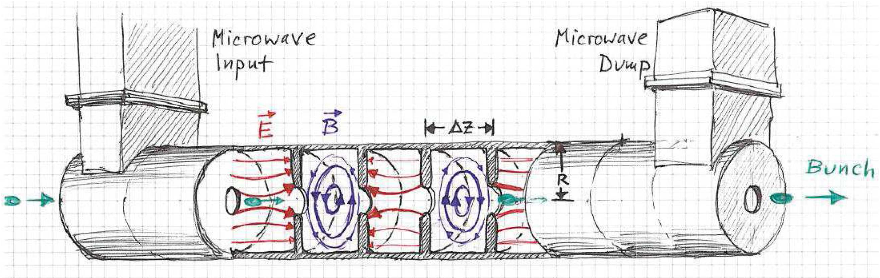
\includegraphics[scale=0.45]{pictures/scheme_ACS}
\caption{Scheme of a travelling wave, disk loaded accelerating structure. In the drawings are visible the input and output couplers, the disk loading the cavity and the beam passing through the irises. From \cite{streun}}
\label{ACS_scheme}

\end{figure}

The accelerating structure is composed by \textit{cells}, which are connected by the \textit{iris} to the other adjacent cells. At the beginning and the end of the structure are present two special cells that are connected to the input and output coupler for the RF. Apart for the cells with the couplers, the structures present a full rotational symmetry on the beam axis.
The role of the irises is creating a free path for the passage of the beam and allowing the propagation of the EM field from the input coupler to the output one. In the case of room temperature cavities the material normally used is Copper, while for superconducting cavities the material can vary and also metallic cavities coated internally with a superconductive layer are a possibility.

From the field perspective, the fact that the accelerating structure is loaded with the disks changes the way that the EM waves propagate in the structure. I won't go through the full mathematical description, which is very detailed in \cite{ Jackson:ClassEM,Weiss:261732}, but simply give a general idea of the process and of the relevant results.

The geometry of the accelerating structure can be seen as a cylindrical cavity loaded regularly with the disks. If as first approximation we consider an infinite structure, it is possible to use the \textit{Floquet's Theorem}, that can be summarised as follows: \textit{"In a given mode of an infinite periodic structure, the fields at two different cross sections that are separated by one period differ only by a constant factor, which in general is a complex number"}. This has two main implications: there are some regions of the spectrum of $\omega$ that don't allow the waves to propagate, called \textit{stopbands}, and others, called \textit{passbands}, where the propagation is allowed with a \textit{phase shift} $\Delta \phi = k_0 d$, where d is the length of the cell. The phase advance per cell is a peculiar parameter of every structure, and is defined in the design phase.

The waves that are allowed to propagate in such conditions are called \textit{Space Armonics}, and can be seen as an infinite number of waves propagating at the same frequency but with different wavenumbers. The dispersion relation becomes
\begin{equation}
\omega ^2 = \omega^2_c + c^2 \left( k_0 + \frac{2\pi n}{d} \right)^2
\end{equation}
where the principal wave of the mode has $n=0$ and the others have $n$ according to the direction of propagation.

The phase velocity of the n-th harmonic becomes
\begin{equation}
\beta_n = \frac{\omega}{k_n c} = \frac{\beta_0}{1+n\beta_0 \lambda/d}
\end{equation}
which allows to reach an arbitrary low phase velocity, as requested for the particle acceleration.

The comparison of the phase velocity of a waveguide and accelerating structure is presented in figure \ref{vp_fig}.



\begin{figure}[h]
\centering

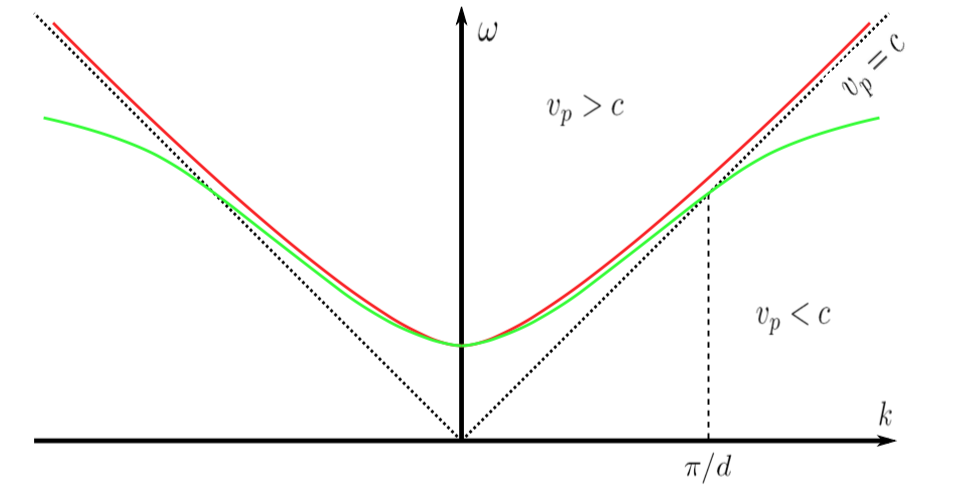
\includegraphics[scale=0.4]{pictures/vp}
\caption{Brillouin diagram of a uniform waveguide (red) compared to a disk-loaded accelerating structure (green) \cite{Kovermann:1330346}}
\label{vp_fig}

\end{figure}


\subsection[Figure of merit for accelerating structures]{Figure of merit for accelerating structures}

To characterize the different accelerating structures, is necessary to rely on some significant quantities that can be derived by the geometry of the cavities. The most important figures of merit (FOMs) are the following (many different definitions are commonly used, here are reported in accordance with \cite{TECKER:RFCAS}):
\begin{itemize}

\item \textbf{Quality factor} 
\begin{equation}
Q_0 = \frac{\omega_0 U}{P_{loss}} 
\end{equation}
is a standard FOM for the resonant cavities, representing the stored energy over the power dissipated

\item \textbf{Shunt impedance} 
\begin{equation}
R = \frac{V_{acc}^2}{2P_{loss}}  \quad [M\Omega]
\end{equation}
represent the effectiveness of producing an axial voltage $V_0$ for a given power dissipated. For long cavities, where is preferable to have a quantity that is independent by the length of the structure, is commonly used the Shunt impedance per unit length

\begin{equation}
Z = \frac{R}{L}  \quad [M\Omega / m]
\end{equation}

where L is the length of the cavity.

\item \textbf{R over Q} 
\begin{equation}
\frac{R}{Q} = \frac{(V_{acc})^2}{2\omega_0 U}  \quad [M\Omega]
\end{equation}
represents the relation between the accelerating field and the stored energy


\item \textbf{Filling time}
\begin{equation}
t_F = \int_0^L \frac{dz}{v_g (z)}
\end{equation}
time needed by the EM field to fill the structure

\item \textbf{Power delivered to the beam}
\begin{equation}
P_B = \frac{I \Delta W}{q}
\end{equation}
where $I$ is the beam current and $\Delta W$ is the energy gain

\item \textbf{Beam loading ratio}
\begin{equation}
\epsilon_s = \frac{P_B}{P_{tot}}
\end{equation}
represents the fraction of power that is delivered to the beam

\end{itemize}


\section[High power limits and scaling laws]{High power limits and scaling laws}

The limiting factors for room-temperature high-gradient accelerators have been identified as \textit{field emission} and \textit{RF breakdown}. The former is the emission of electrons in the form of the so called \textit{"Dark current"}, that subtracts RF power, causes radiation and can produce wakefields; the latter is a limiting factor to the operation of accelerators and can damage the structures.\cite{Wang:1997ip}

The understanding of these phenomena is particularly challenging and requires a mixture of notions of disciplines such as surface physics, metallurgy, fabrication processes, microwaves, beam dynamic and plasma physics. At the moment a satisfactory unified theory of the processes that take place during the breakdowns have not been found yet, then the improvement of the structures is achieved using some scaling laws for the high power limitations, that have been deducted from the experience and the experiments on the structures tested so far. 


\subsection[Field emission law]{Field emission law}

\subsubsection{Emission from flat clean surface}

The field emission law was theorised by Fowler and Nordheim in 1928 and rule the current emission from a metal with applied an intense electric field. The derivation was carried on calculating the tunnel probability of electrons of the conduction band through the perfectly flat and clean surface of a metal. \\The applied electric field modify the potential barrier, and the current density of emitted electrons can be derived as the following, giving the  \textit{Fowler-Nordheim equation} \cite{Fowler173}
\begin{equation}
J_F = \frac{ 1.54\times10^{-6} \times 10^{4.52\phi^{-0.5}} E^2}{  \phi } \, \text{exp} \left ( -\frac{6.53\times 10^9 \phi^{1.5}}{E} \right ) \quad [A\,m^{-2}]  \label{FNlaw}
\end{equation}
where $\phi$ is the work function of the material and $E$ is the applied electric field.

\subsubsection{Enhanced field emission}

It's well known that almost any surface is never perfectly clean and flat, and also the fact that the asperities of the surface provoke an enhancement of the local electric field. This behaviour lead to the phenomenon known as \textit{Enhanced Field Emission} (EFE), which major contributors are:
\begin{itemize}
\item Surface imperfection due to imperfect machining
\item Metallic dust
\item Molten craters after breakdowns
\item Absorbed gas
\end{itemize} 
and some others. These effects can create particular sites known as "emitters". It's a common praxis define the field enhancement factor $\beta$ to relate the electric field to the microscopic one
\begin{equation}
E_{m} = \beta E
\end{equation}
and the $\beta$ factors can be calculated according to the emitter's geometry \cite{Rohrbach:190223} as exploited in figure \ref{tip_factors}.
Once the local field is known, using the formula \ref{FNlaw} calculate the current emitted from EFE by an emitter site of area A gives 
\begin{equation}
I_F = \frac{ 1.54\times10^{-6} \times 10^{4.52\phi^{-0.5}} A \beta^2 E^2}{  \phi } \, \text{exp} \left ( -\frac{6.53\times 10^9 \phi^{1.5}}{\beta E} \right ) \quad [A]  \label{If}
\end{equation}
where $\beta E$ is the local field, $\phi$ is the work function of the material and $A$ the area of the considered emitter.

 In the RF case the average current emitted is given by similar calculations, averaging the electric field on an RF period  \cite{Wang:1997ip}. 

Experimental evidence of the dark current emission have been detected by setups equipped with Faraday Cups, as in \cite{Wuensch:advaces}.

The emission of dark current seems to be a precursor of the breakdown  process, even if the relationship between the two processes has not been clarified so far.

\begin{figure}[h]
\centering

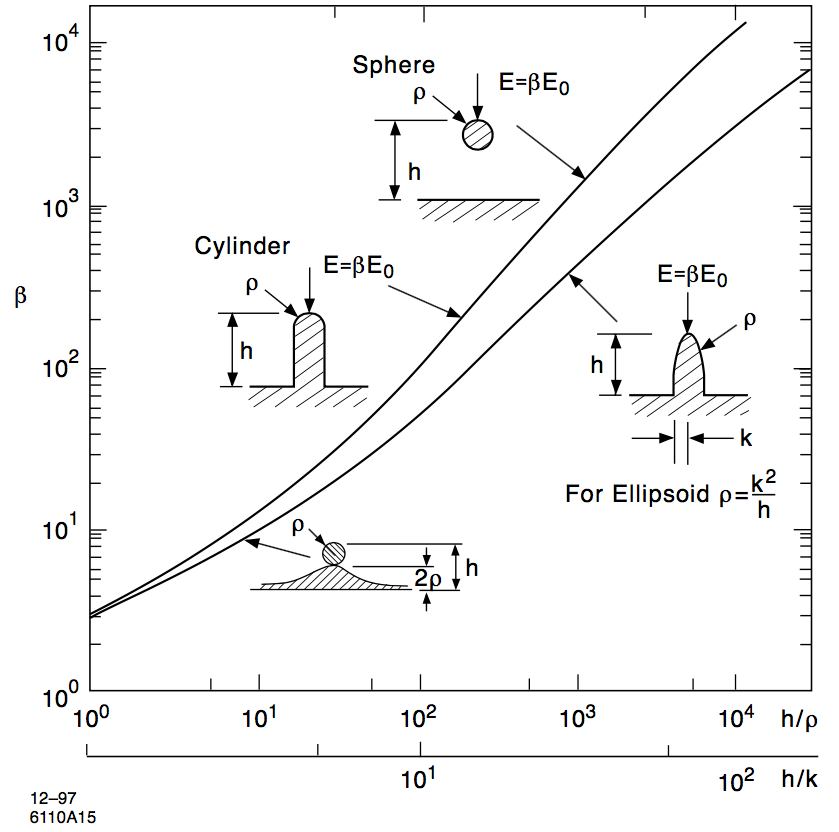
\includegraphics[scale=0.3]{pictures/beta_tip_val}
\caption{Field enhancement factors for simple geometries of metallic protrusions, plotted as function of geometrical features. From \cite{Rohrbach:190223}}
\label{tip_factors}

\end{figure}


%%%%%% EXCURSUS ABOUT REASONABLE VALUES OF BETA




\subsection[Kilpatrick's critereon]{Kilpatrick's critereon}

The Kilpatrick's Critereon was the first attempt to create a high power limit for the vacuum breakdown valid both in DC and RF applications \cite{KilpLimit}. The model was based on the acknowledgement of the Field Emission, and suggesting that the vacuum arc was created by the cascade of secondary electrons ejected from the surface by ion bombardment.

Using data collected in the 1950's, the following empirical law was formulated
\begin{equation}
W E^2 \text{exp} \left (  -1.7\times 10^5 E^{-1}  \right ) = 1.8 \times 10^{14}
\label{KilpLaw}
\end{equation}
where $W$ is the maximum possible ion energy in $eV$, and $E$ is the field in $V/m$. This can also be rewritten in the case of the RF to give a frequency limit, as
\begin{equation}
f = 1.64 \,\, E^2 \,\, \text{exp} \left (  -\frac{8.5}{E} \right )
\end{equation}
where $f$ is the frequency in $MHz$ and $E$ is the electric field in $MV/m$.

\begin{figure}[h]
\centering

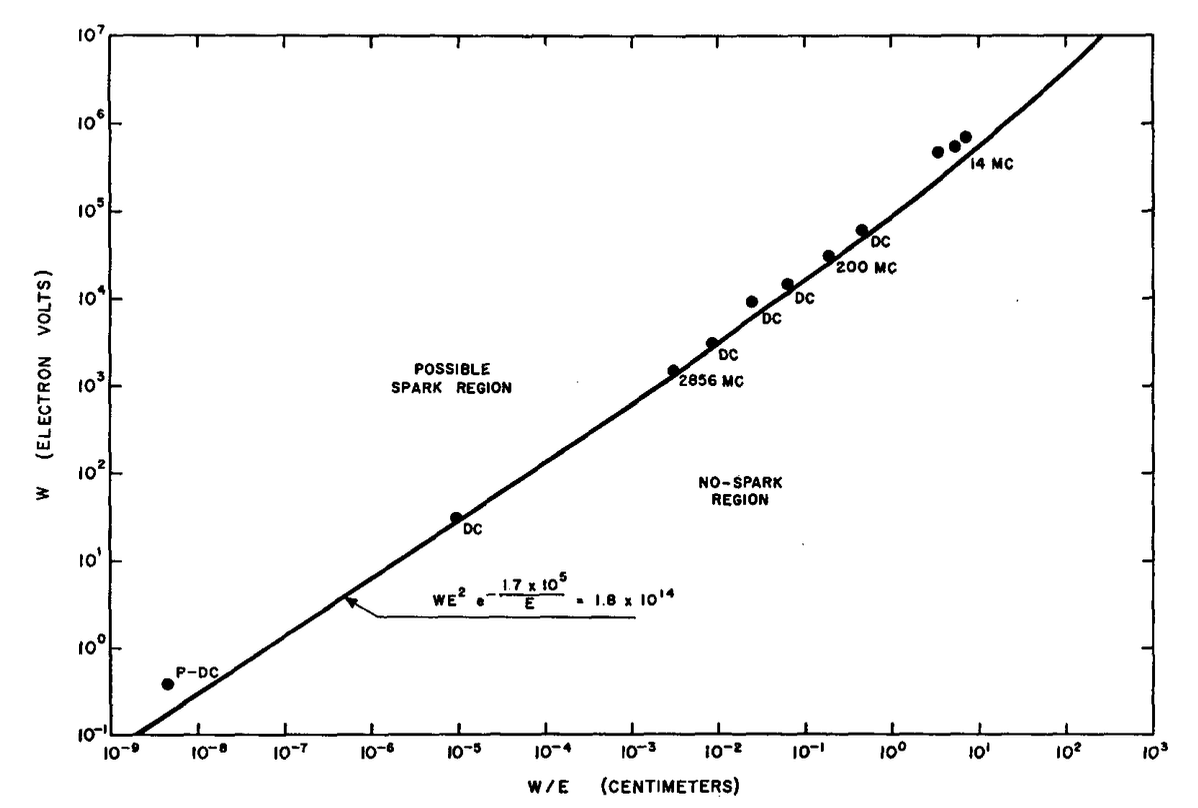
\includegraphics[scale=0.4]{pictures/kilpatrickCrit}
\caption{Kilpatrick's original plot. Note that $MC = MHz$ (\textit{Mega Cycles}) and that $W$ for RF is function of frequency, voltage and gap amplitude.\\ See paper for details  \cite{KilpLimit}}
\label{kilpPlot}

\end{figure}

The critereon was reviewed many times up to now, because the experiments conducted nowadays show a limit up to 10 times lower than Kilpatrick's prediction, and this can be addressed to different reasons: first of all the quality of the machining of the structures have increased considerably since the 1950's; in second instance the formula for $W$ was deducted for parallel plates, but the condition inside the RF cavities are different during operations; and finally the key assumption was that the breakdown was triggered by the secondary emission provoked by the ion bombardment.

%%%%% GOOD OF KILPATRICK --> BD and FIELD EMISSION ARE PROVOKED BY DIFFERENT PHENOMENA

At the end of the 1980's J.D.Wang finally proposed a model based on microprotrusion effect on the field and field emission, that involves the formation of a micro-plasma during the breakdown process. Also the Kilpatrick's limit was revised again in order to match the experimental results. \cite{Wang:1986, kilp:story}


\subsection[Power flow based criteria]{Power flow based criteria}

Other scalings have been proposed, like the phenomenological $P/C$-criterion, where $P$ is the power flowing in the cavity and $C$ the minimum iris circumference. It's straightforward to see that this is strongly related to the maximum surface electrical field, which is stronger for smaller irises. Also have to be underlined that this is suitable just to travelling wave structures (TWS), since the power flow in standing wave structures (SWS) is close to zero. 

In recent years a more advanced version of the scaling have been presented \cite{Wuensch:932674}, which is quantified by
\begin{equation}
\frac{P \tau^{1/3}}{C}
\end{equation}
where $P$ is the power flow through the structure, $\tau$ the pulse length and $C$ the minimum iris circumference. This has also been formulated as $(f \times P/C )^{0.5}$, which is a quantity linear with the field \cite{Wuensch:1004189}.

Anyway, although these criteria are still in use today for the accelerating structure design, finding a more general criterion valid for any type of cavity is necessary.

\subsection{The modified Poynting vector $S_c$}

During the development of high gradient normal conducting accelerating structures for the CLIC project, was developed a new field quantity, the \textit{Modified Poynting Vector} $S_c$, that is suitable both for TWS and SWS. \cite{Grudiev:newLoc}

The formulation is based on two assumptions: the breakdown process is a determined by the accumulation of the pulses rather than the single pulse and the possible triggers of the breakdown can be induced by many processes that will be discussed later and are not relevant for the scaling law derivation.

A number of effects have to be taken into account (a simple geometry is considered, a cilindrical protrusion surmounted by a emispherical cap): 

\subsubsection{Pulsed heating by field emission current}

it's known that the field emission gets enhanced by the presence of the protrusion as described before, and in this case the field enhancement factor can be expressed as $\beta \simeq h/r$, where $h$ is the tip height and $r$ is the cap radius. So the tip will emit a current according to the Fowler-Nordheim law \ref{If}, causing in first approximation the heating of the tip due to the ohmic heating as shown in figure \ref{figure_S_c}. Assuming that the edge of the tip will be the most heated part, and using the heat conduction equation, it is possible to derive the emitted current to bring the tip to the melted state, which is found to be approximately $36\, A/\mu m^2$ for a tip of $1 \, \mu m$ height and a pulse of $100\, ns$. This is consistent with the findings in \cite{soviet:1983}. The $\beta$ factor can be then derived, which is approximately between 40 and 60 considering a surface electric field in case of breakdown between 200 and 300 $MV/m$, in according with the experimental results.

 \begin{figure}
 \centering
 \subfigure[Electric field distribution]
   {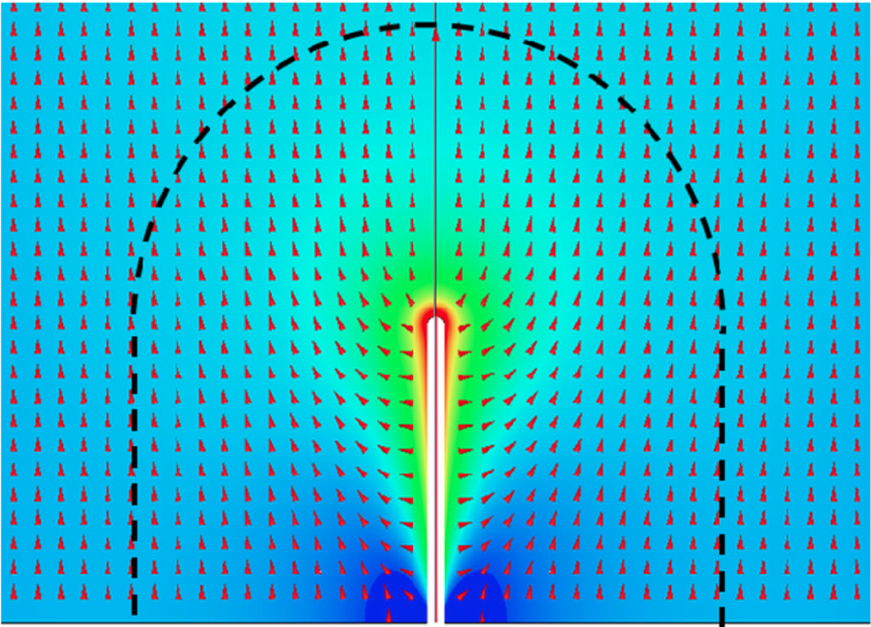
\includegraphics[width=6cm,height=5cm]{pictures/field_S_c}}
 \hspace{5mm}
 \subfigure[Field emitted power flow]
   {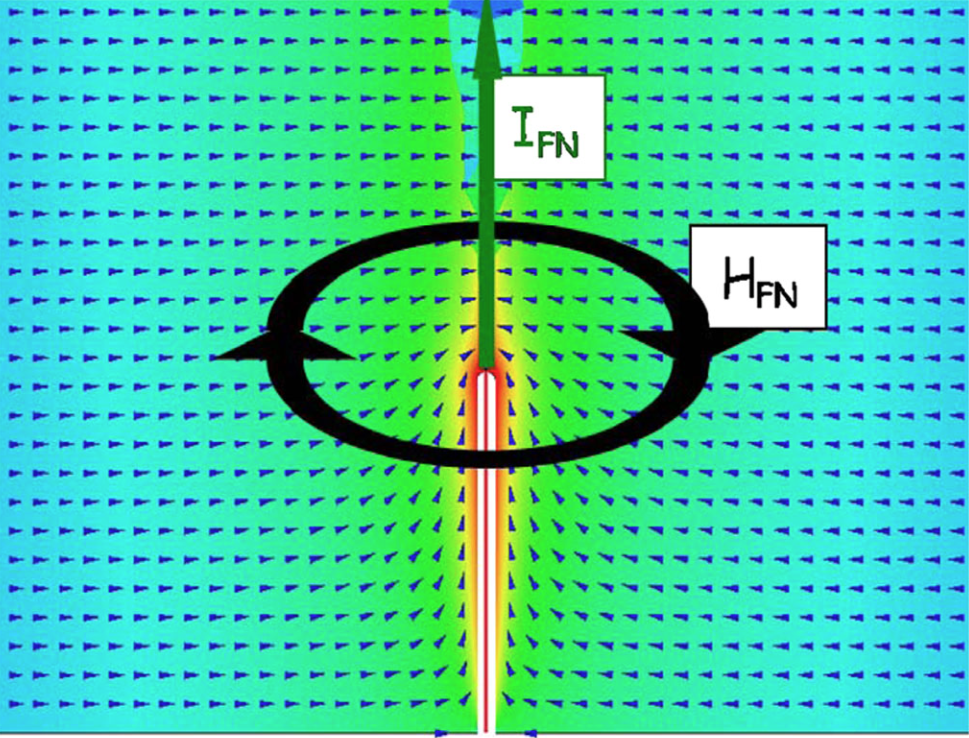
\includegraphics[width=6cm,height=5cm]{pictures/S_c_FEM}}
 \caption{(a) Electric field distribution around the protrusion considered. (b) Field emitted current and power flow. In both the plots arrows indicate the direction of the field and the color code the absolute value of the field, mapped logarithmically.\cite{Grudiev:newLoc} }
 \label{figure_S_c}
 
 \end{figure}



\subsubsection{Power flow near an emission site}

The heating of the tip mentioned before requires a huge amount of energy, which can be supplied only by the RF power present into the cavity. This is described by the Poynting vector $S_{RF} = E\times H_{RF}$. As discussed before a current is established in the tip, and flows through, subtracting energy to the EM field in the surroundings of the tip. The current flows through the tip and leave it at the edge, getting sprayed in the cavity according to the Fowler-Nordheim theory. Since any current flowing creates an associated magnetic field, the power flow due to the emission is given by $S_{FN}=E\times H_{FN}$. 

The key point is that since the copper is a very good conductor, to provoke a notable ohmic heating of the tip, a significant power flow through the tip is necessary. This can be calculated evaluating the $S_{FN}$ at a distance $d=h$ from the edge of the tip, where the electric field is not perturbed anymore by the shape of the tip itself. This can be formulated as the condition 
\begin{equation}
P_{RF} \ge P_{FN} \gg P_{loss}
\end{equation}
where $P_{loss}$ is the power lost for ohmic heating and $P_{FN}$ the power flow through the tip.

Considering now the relative phase of the $P_{RF}$ and of the $P_{FN}$ it is possible to derive an expression for the power emitted from the tip in a copper cavity
\begin{equation}
P_{FN} (t) = A \, E^3_0 \, sin^3 \omega t \,  \, exp \left ( \frac{-62}{\beta E_0 \, sin \, \omega t} \right )
\end{equation}
where have been used the work function for the copper $\phi = 4.5 \, eV$, $A$ is the area of the conductor and $\omega = 2 \pi f$ is the angular velocity.

The RF power can be divided in real and imaginary part, with a phase shift of $90^\circ$. The real part is the energy propagating into the structure only and the imaginary part is the energy stored in the cavity both magnetically or electrically as happens in every resonant cavity. Since the active power flow is more efficient than the reactive one in providing power for the field emission, a weighting factor $g_c$ is introduced. Also for practice reasons since all the simulation codes work using the complex Poynting vector $\bar{S}$, the precedent reasoning can be adapted to meet the custom, using the \textit{Modified Poynting Vector}
\begin{equation}
S_c = Re\{ \bar{S} \} + g_c \, Im \{ \bar{S} \} \qquad [W/\mu m^2]
\end{equation} 

Since this quantity can be calculated in any point of a structure, this allows to identify in advance the regions which are more sensible to the breakdown process. The rule of thumb given by the experience says that this quantity should not exceed the value of $5 W/\mu m^2$ to have a breakdown rate smaller than $1\times 10^{-6} \, bpp \, m^{-1}$ with a pulse length of 200 ns.

This quantity have been used successfully to design all the last generations of CLIC structures, including the one tested in this work.






\section[The TD26CC structure for the Main Beam of CLIC]{The TD26CC structure for the Main Beam of CLIC}

After the precedent part about the general laws that regulate the operation of the TWS, now will be presented the structure under test in this work, the TD26CC, which stays for Tapered, Damped, 26-cells active cells structure with Compact Couplers.

It's necessary to keep present in mind that in the design of the real cavities, it's almost never possible to use the general laws described in precedence because of the high complexity of the geometries. A great work of design and simulation is necessary then, and is carried out with complex numerical simulations. In this section will be presented a summary of the parameters and features of the cavity, the details can be found in \cite{CLIC:cdr,Grudiev:td26cc,Lunin:1333709}.

As pointed out in \cite{CLIC:cdr}, the main constraints in the structures for the main beam LINAC are 
\begin{enumerate}
\item Maximum surface electric field: $E_{surf}^{max} < 260 \, MV/m$
\item Pulsed surface heating: $\Delta T^{max} < 56 \,K$
\item Power density: $P_{in}/C\tau_p^{1/3} < 18 MW/mm \, ns^{1/3}$
\end{enumerate}

These limitations, together with the parameters listed in the section 1.2.2, brought to the current design after a long simulation and tradeoff of the parameters. The main parameters are reported in Table \ref{TD26_param_1}

\begin{table}[h]
  \centering
    \begin{tabular}{ l l  }
    \hline
    \hline
    Average loaded accelerating gradient			& $100\, MV/m$	\\
    Frequency								& $12 \, GHz$	\\        
    RF phase advance per cell					& $2/3 \, \pi \, rad$	\\       
    Average iris radius to wavelength ratio			& $0.11$	\\ 
    Input, output iris radii      					& $3.15, \, 2.35 \, mm$	\\
    Input, output iris thickness      				& $1.67, \, 1.00 \, mm$	\\
    Input, output group velocity					& $1.65, \, 0.83 \, \% \text{ of }c $	\\
    First, last cell Q-factor						& $5536,\,5738$\\
    First, last cell shunt impedance				& $81,\,103\, M\Omega / m$\\
    Number of regular cells						& $26$	\\   
    Structure length including couplers			& $230 \,mm$	\\   
    Filling time								& $67 \, ns$	\\               
    Total pulse length							& $242 \, ns$	\\      
    Peak input power 							& $61.3 \, MW$	\\        
    RF-to-beam efficiency						& $27.7 \%$	\\   
    Maximum surface electric field				& $230 \, MV/m$	\\           
    Maximum pulsed surface heating				& $47 \, K$	\\       
    \hline
    \hline
    \end{tabular}
  \caption{Parameters of the structure}
\label{TD26_param_1}
\end{table}

 \begin{figure}[h]
 \centering
 \subfigure[A disk composing the structure]
   {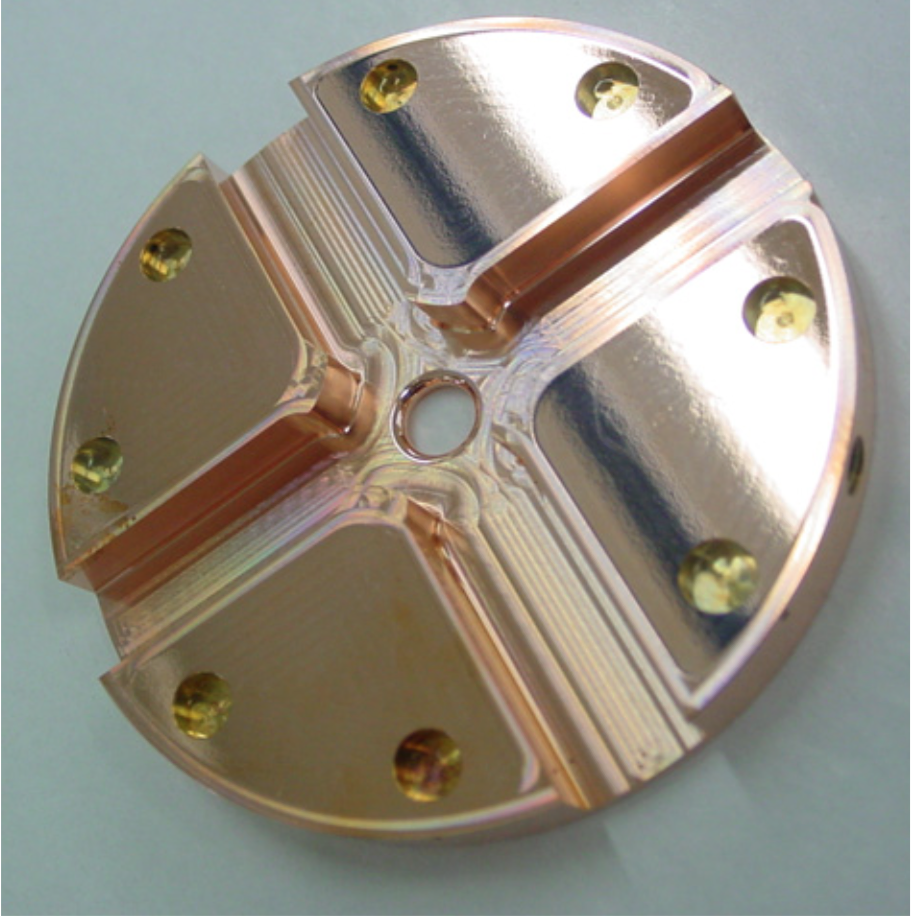
\includegraphics[scale=0.16]{pictures/photo_disk}}
 \hspace{5mm}
 \subfigure[CAD model of the structure, open to show the damping material]
   {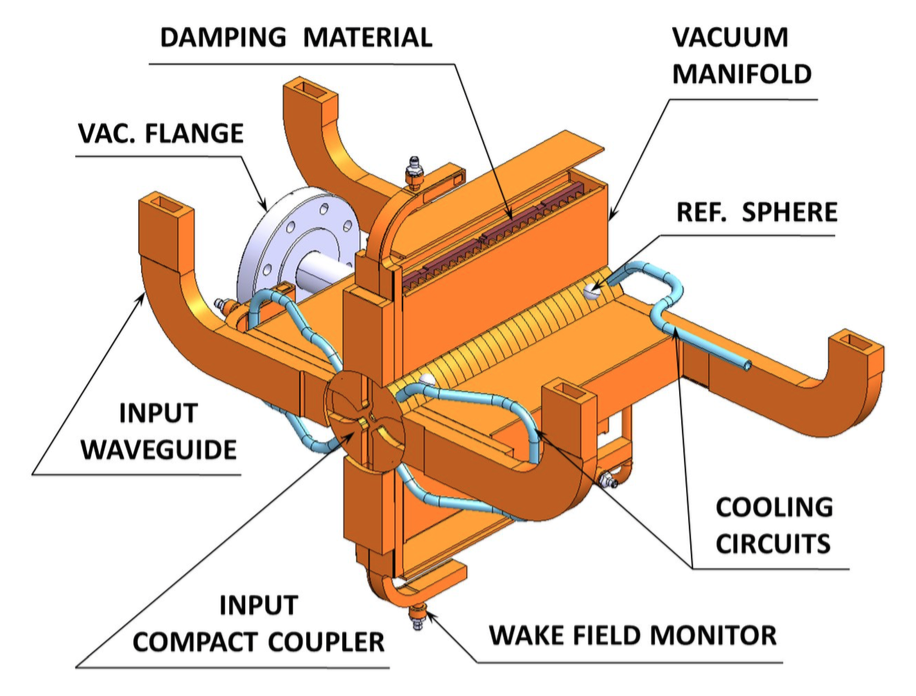
\includegraphics[scale=0.22]{pictures/TD26_layout}}
 \caption{A disk composing the structure (left) and the scheme of an accelerating structure (right), including couplers for the RF, cooling elements and connection flanges. The wakefield monitor is not present in the prototype under test}
 \label{CLICdisk}
 
 \end{figure}
 
The structure is realised stacking machined copper disks that are then brazed together with a particular procedure that have been elaborated in order to achieve the highest mechanical precision possible in the alignment of the parts. In figure \ref{CLICdisk} are shown a disk and a model of the accelerating structure.

The iris radius and thickness are linearly tapered in order to optimise the various high power parameters and avoid the presence of 'hot spots' along the structure. 

Because of the high number of bunches per train and of the very short spacing between them (see table 1.1), the structure is realised in order to extract the transverse wakefields that can develop in the structure. This is realised using 4 symmetrical waveguides of dimensions carefully selected in order to allow the propagation of just the higher order electromagnetic modes (HOMs) but not the fundamental one that is used to accelerate the bunches and is provided from the input couplers. Once extracted, the transverse wakefields are dumped on tips of Silicon Carbide (SiC) that are placed at 50 mm of distance from the axis of the cavity.
The tapering also provide detuning of the high order modes, which are an issue even for highly damped structures.

In the structure are also installed the cooling water circuits and the vacuum flanges. The "CC" in the initials of the cavity name refers in fact to the particular type of vacuum flanges used for this structure.

\begin{figure}[h]
\centering

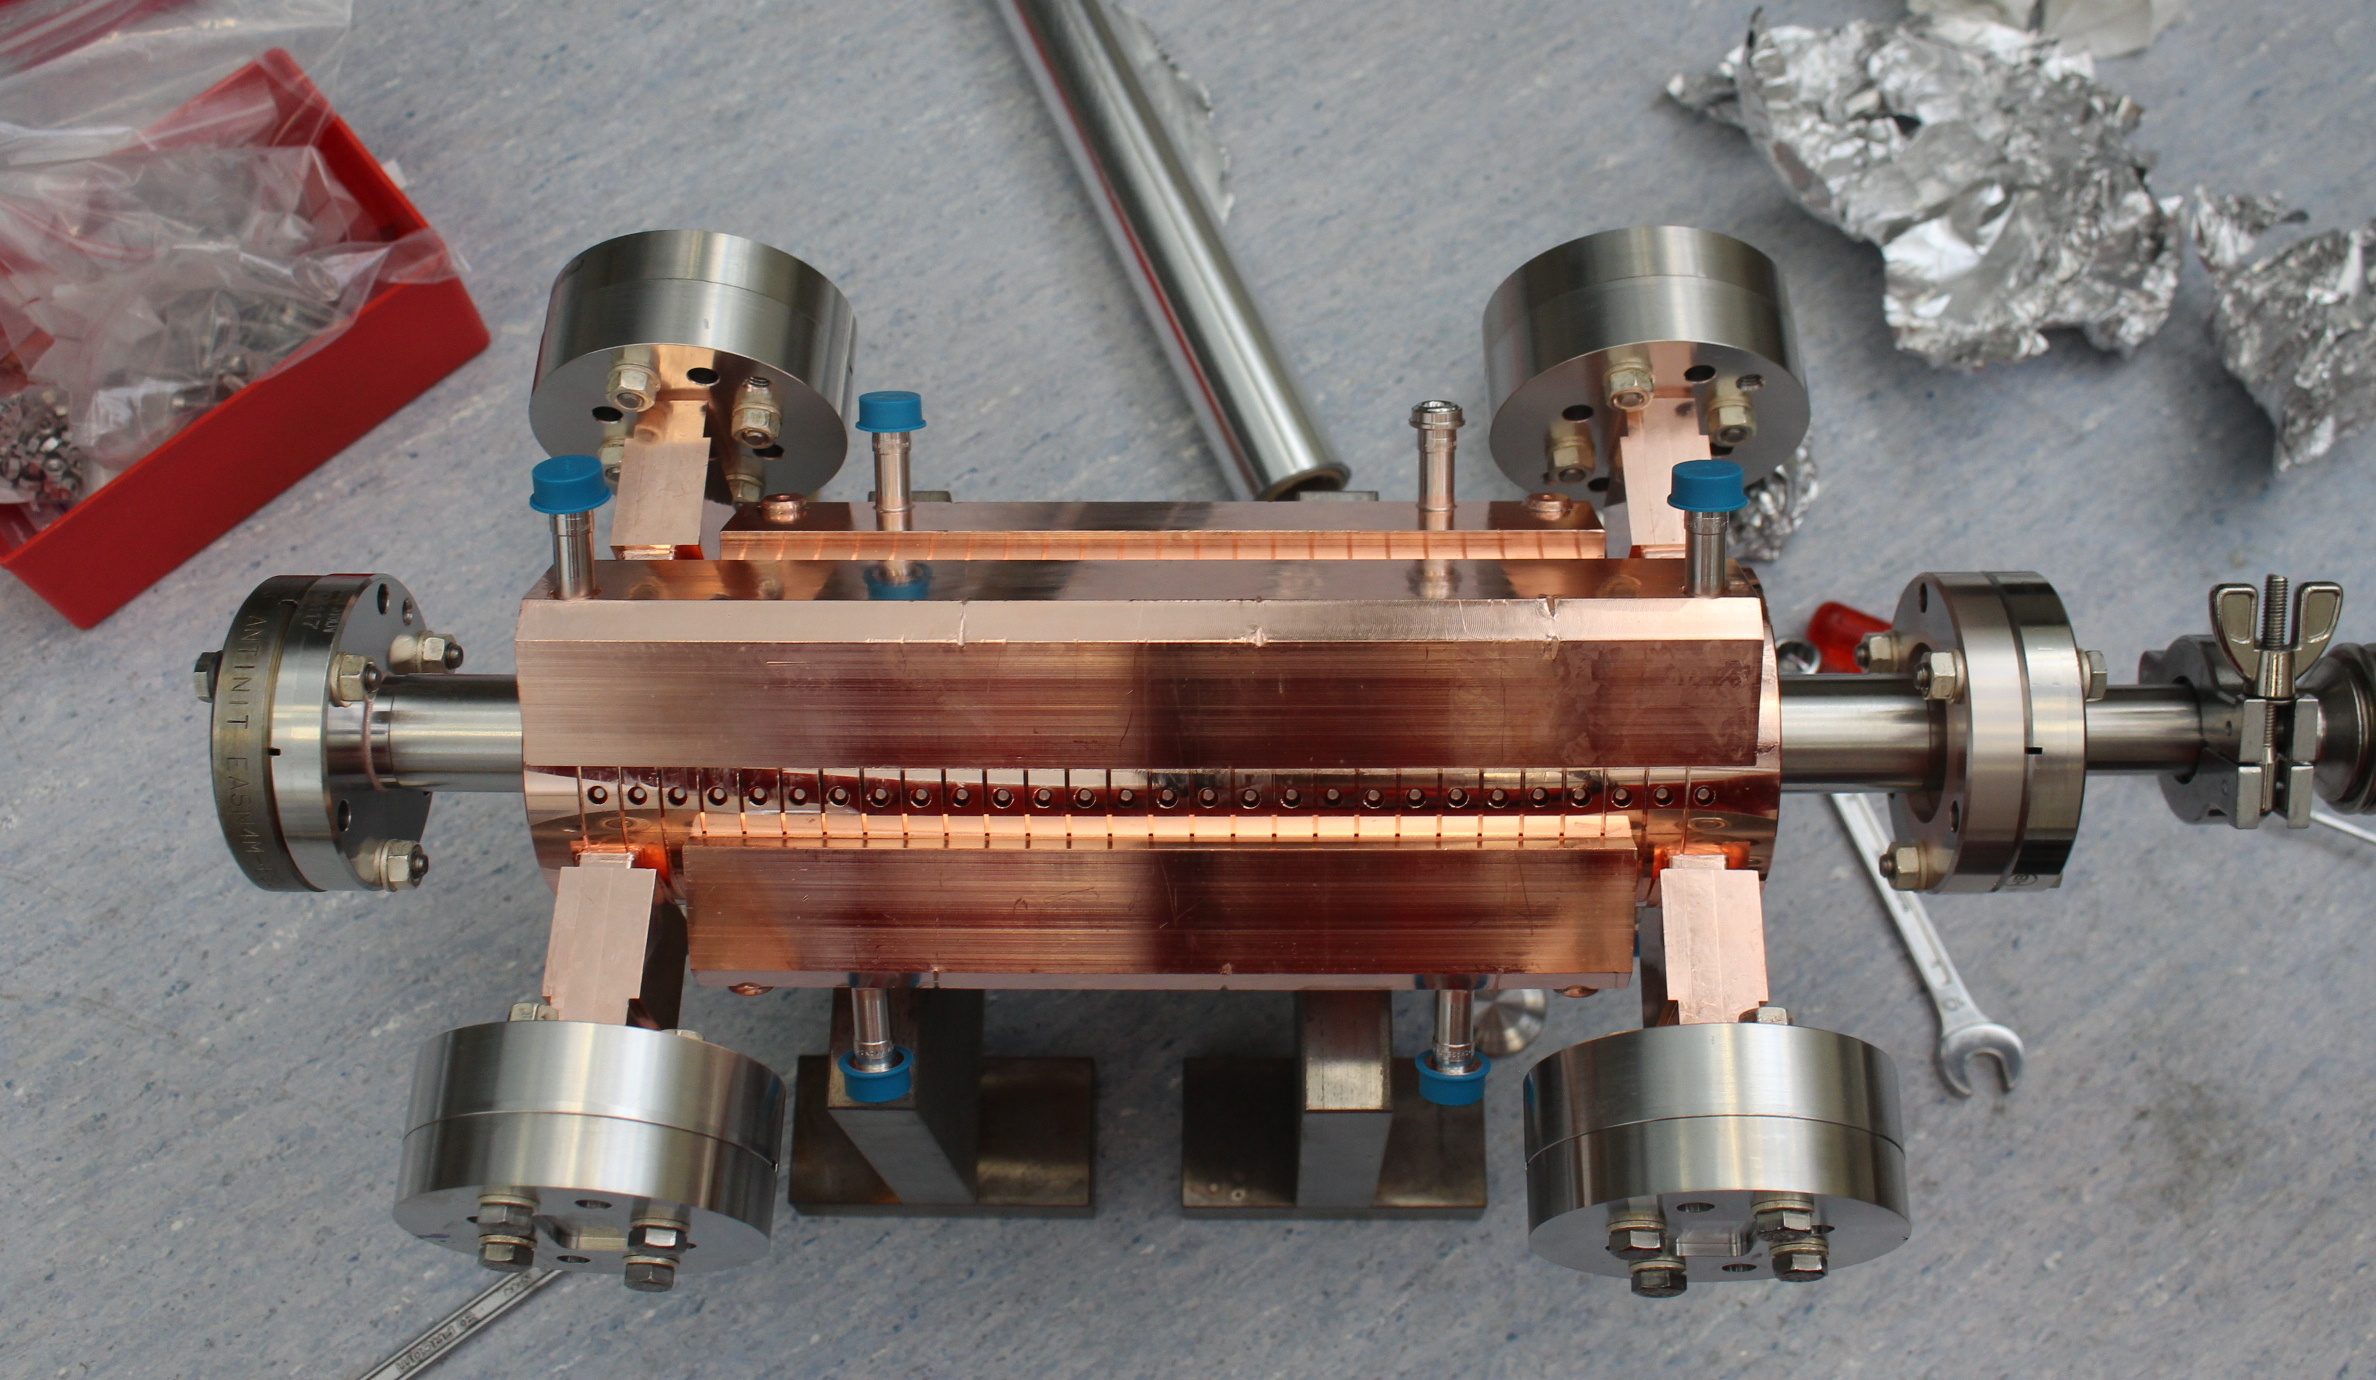
\includegraphics[scale=0.16]{pictures/td26_test_photo}
\caption{The structure prototype before the installation \textit{(Photo A. Solodko)}}
\label{td26_test_photo}

\end{figure}


